\documentclass[a0,portrait]{a0poster}

% =====================================================================
%  PACKAGES
% =====================================================================
\usepackage[left=4cm,right=4cm,top=4cm,bottom=4cm]{geometry}
\usepackage[svgnames,table]{xcolor}
\usepackage{times}
\usepackage{graphicx}
\graphicspath{{figures/}}
\usepackage{booktabs}
\usepackage[font=small,labelfont=bf]{caption}
\usepackage{amsfonts,amsmath,amsthm,amssymb}
\usepackage{subcaption}
\usepackage{sectsty}
\usepackage{tikz}
\usepackage{pgfplots}
\pgfplotsset{compat=1.18}
\usepackage{adjustbox}
\usepackage{array}
\usepackage{tabularx}
\usepackage{colortbl}
\usepackage{mdframed}
\usepackage{enumitem}
\usepackage{microtype}

% =====================================================================
%  TikZ LIBRARIES
% =====================================================================
\usetikzlibrary{
  arrows.meta,
  shapes.geometric,
  positioning,
  fit,
  backgrounds,
  decorations.pathreplacing,
  calc
}

% =====================================================================
%  COLOR PALETTE
% =====================================================================
\definecolor{PosterNavy}  {RGB}{10,38,71}
\definecolor{PosterRed}   {RGB}{180,20,20}
\definecolor{PosterBlue}  {RGB}{0,102,179}
\definecolor{PosterTeal}  {RGB}{0,139,139}
\definecolor{PosterOrange}{RGB}{230,100,20}
\definecolor{PosterGray}  {RGB}{245,245,248}
\definecolor{PosterGreen} {RGB}{40,140,60}

% =====================================================================
%  FONT & SECTION STYLING
% =====================================================================
\sectionfont{\Large\color{PosterNavy}\bfseries}
\renewcommand{\familydefault}{\sfdefault}

% =====================================================================
%  HELPER: shaded info-box
% =====================================================================
\newenvironment{infobox}[1][PosterGray!60]{%
  \begin{mdframed}[backgroundcolor=#1,linecolor=PosterNavy,linewidth=1.2pt,
    innertopmargin=6pt,innerbottommargin=6pt,
    innerleftmargin=8pt,innerrightmargin=8pt,roundcorner=4pt]
}{%
  \end{mdframed}
}

% =====================================================================
%  DOCUMENT
% =====================================================================
\begin{document}

% ─────────────────────────────────────────────────────────────────────
%  HEADER
% ─────────────────────────────────────────────────────────────────────
\noindent\begin{minipage}[b]{0.13\linewidth}
  
\includegraphics[width=\linewidth]{iyte-logo.png}
\end{minipage}
\hspace{0.02\linewidth}
\begin{minipage}[b]{0.72\linewidth}
  \begin{center}
    \Huge\color{PosterRed}\textbf{Multi-Criteria Optimization of Electric Vehicle\\[4pt]
    Charging and Route Planning}\color{black}\\[0.5cm]
    \huge\textbf{• Ata T\"{u}rky{\i}lmaz (300201055)
                 \quad • Yusuf Celal Zeybek (310201105)}\\[0.3cm]
    \LARGE Advisor: Prof.\ Dr.\ C\"{u}neyt F.\ Bazlama\c{c}c{\i}
           $\mid$ Computer Engineering, IZTECH
  \end{center}
\end{minipage}
\hspace{0.02\linewidth}

\vspace{1cm}
\rule{\linewidth}{3pt}
\vspace{1cm}

% ─────────────────────────────────────────────────────────────────────
%  THREE-COLUMN BODY
% ─────────────────────────────────────────────────────────────────────
\noindent\begin{minipage}[t][83cm]{0.31\linewidth}

% ── SECTION 1 ────────────────────────────────────────────────────────
\section*{1.\ Motivation \& Problem Definition}
\normalsize
Commercial navigation tools evaluate shortest paths statically, ignoring EV
battery physics, charging curves, and weather.  Academic models focus on
corporate \emph{fleets}, ignoring individual drivers.

We formulate the \textbf{Multi-Criteria EVCRP} to personalise routes based on
three user-tuneable priority weights:

\begin{itemize}[leftmargin=1.4em,itemsep=2pt]
  \item \textbf{Time ($w_1$):}    Driving + queue + non-linear charging delay.
  \item \textbf{Cost ($w_2$):}    Financial tariffs across charging operators.
  \item \textbf{Anxiety ($w_3$):} Safety buffers above critical battery floors.
\end{itemize}

\vspace{0.4cm}
Our global objective minimizes the weighted criteria:
\[
  Z = w_1 \cdot \text{Time} + w_2 \cdot \text{Cost} + w_3 \cdot \text{Anxiety}
\]

% ── SECTION 2 — SYSTEM ARCHITECTURE DIAGRAM ──────────────────────────
\section*{2.\ System Architecture}

\begin{center}
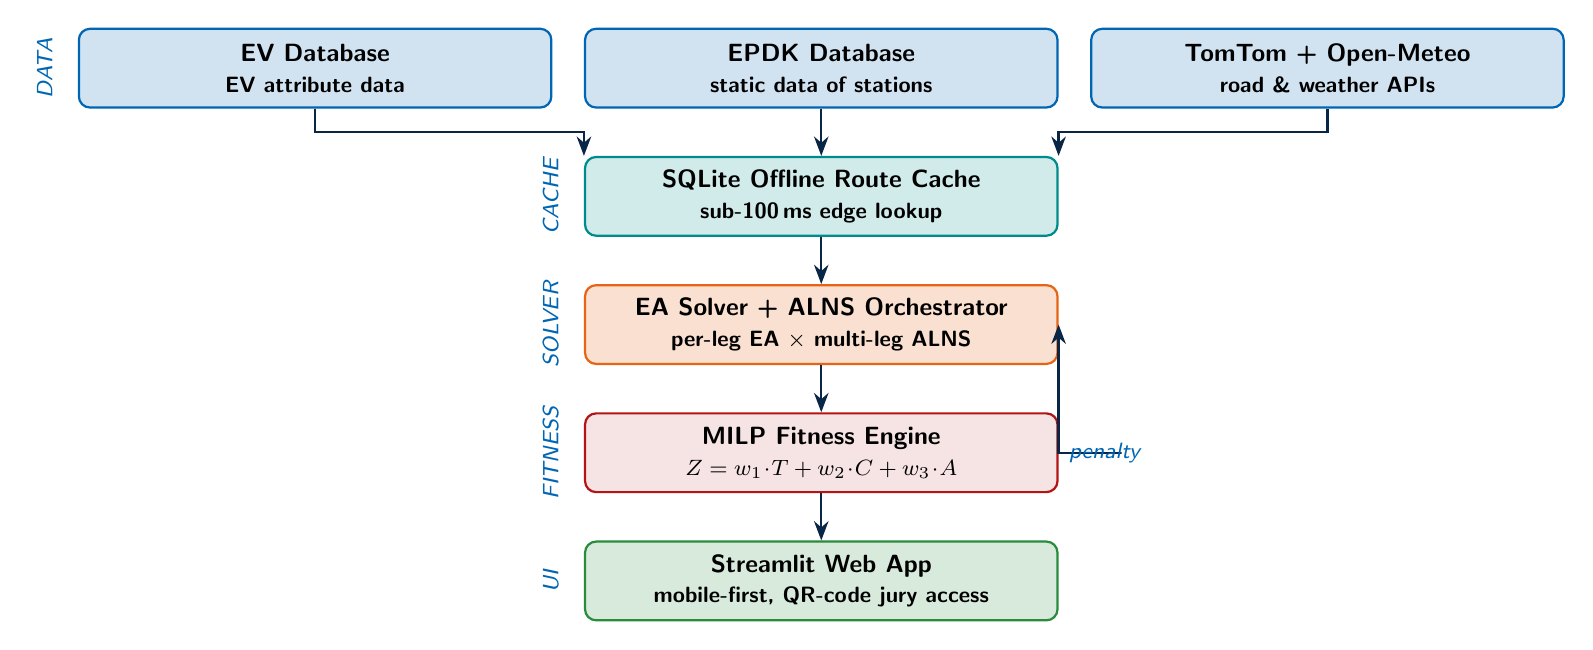
\begin{tikzpicture}[
  node distance=0.55cm,
  box/.style={rectangle, rounded corners=4pt, minimum width=6.0cm,
              minimum height=1.0cm, align=center, font=\small\bfseries,
              draw, thick},
  arr/.style={-{Stealth[length=7pt]}, thick, color=PosterNavy},
  lbl/.style={font=\footnotesize\itshape, color=PosterBlue}
]

\node[box, fill=PosterBlue!18, draw=PosterBlue]   (epdk)
      {EPDK Database\\ {\footnotesize static data of stations}};

\node[box, fill=PosterBlue!18, draw=PosterBlue,
      right=0.4cm of epdk]                         (apis)
      {TomTom + Open-Meteo\\ {\footnotesize road \& weather APIs}};

\node[box, fill=PosterBlue!18, draw=PosterBlue,
      left=0.4cm of epdk]                         (evdb)
      {EV Database\\ {\footnotesize EV attribute data}};

\node[box, fill=PosterTeal!18, draw=PosterTeal,
      below=0.6cm of epdk]                         (cache)
      {SQLite Offline Route Cache\\ {\footnotesize sub-100\,ms edge lookup}};

\node[box, fill=PosterOrange!20, draw=PosterOrange,
      below=0.6cm of cache]                        (ea)
      {EA Solver + ALNS Orchestrator\\ {\footnotesize per-leg EA $\times$ multi-leg ALNS}};

\node[box, fill=PosterRed!12, draw=PosterRed,
      below=0.6cm of ea]                           (milp)
      {MILP Fitness Engine\\ {\footnotesize $Z = w_1\!\cdot\!T + w_2\!\cdot\!C + w_3\!\cdot\!A$}};

\node[box, fill=PosterGreen!18, draw=PosterGreen,
      below=0.6cm of milp]                         (ui)
      {Streamlit Web App\\ {\footnotesize mobile-first, QR-code jury access}};

\draw[arr] (epdk.south)  -- (cache.north);
\draw[arr] (evdb.south)  -- ++(0,-0.3) -| (cache.north west);
\draw[arr] (apis.south)  -- ++(0,-0.3) -| (cache.north east);
\draw[arr] (cache) -- (ea);
\draw[arr] (ea)    -- (milp);
\draw[arr] (milp.east) -- ++(0.8,0) -| (ea.east)
           node[lbl, midway, right]{penalty};
\draw[arr] (milp)  -- (ui);

\node[lbl, left=0.2cm of evdb,  rotate=90, anchor=south] {DATA};
\node[lbl, left=0.2cm of cache, rotate=90, anchor=south] {CACHE};
\node[lbl, left=0.2cm of ea,    rotate=90, anchor=south] {SOLVER};
\node[lbl, left=0.2cm of milp,  rotate=90, anchor=south] {FITNESS};
\node[lbl, left=0.2cm of ui,    rotate=90, anchor=south] {UI};

\end{tikzpicture}
\end{center}

\vspace{0.2cm}

% ── SECTION 3 — DATA MODALITIES ──────────────────────────────────────
\section*{3.\ Data Modalities}
\begin{itemize}[leftmargin=1.4em,itemsep=1pt]
  \item \textbf{Live Streams:}    TomTom routing \& Open-Meteo weather ($F_{ext}$).
  \item \textbf{Static Caches:}   EPDK database (14{,}825 plugs) + EV spec tables.
  \item \textbf{Offline SQLite:}  Pre-fetched road edges, enables sub-3\,s solver.
  \item \textbf{Mock Metrics:}    Dynamic pricing ($c_q$) \& queue delays $L_i(t)$.
  \item \textbf{Stress Layers:}   Seeded randomised weather fields.
\end{itemize}

% ── SECTION 4 — EA + ALNS ────────────────────────────────────────────
\section*{4.\ EA\,+\,ALNS Hybrid Solver}
\normalsize

\begin{infobox}
\textbf{Tier 1 --- Per-leg Evolutionary Algorithm (EA)}\\[4pt]
Chromosome encodes routing sequence, charge amounts \emph{and} a
continuous \textbf{velocity gene} $v_i$:
\[
  \bigl[w_0 \!\to\! (s_1,\,q_1,\,\mathbf{v_1}) \!\to\! \cdots \!\to\!
        (s_n,\,q_n,\,\mathbf{v_n}) \!\to\! w_K\bigr]
\]
$v_i \!\in\![0.7,1.3]$; consumption scales as
$E = E_\text{eco}\cdot v_i^{1.6}$ (aero-drag model);
speed capped by TomTom real-world limits.
\end{infobox}

\vspace{0.1cm}

\begin{infobox}[PosterBlue!10]
\textbf{Tier 2 --- Multi-leg ALNS Orchestrator (\texttt{pipeline.py})}\\[3pt]
Manages SOC hand-offs between legs, ensuring global feasibility across
all waypoints via Adaptive Large Neighbourhood Search.
\end{infobox}

\vspace{0.8cm}

\renewcommand{\arraystretch}{1.2}
\small
\begin{tabularx}{\linewidth}{@{}lX@{}}
\toprule
\textbf{EA Parameter}    & \textbf{Value}\\
\midrule
Population $P$           & 60 individuals\\
Init strategy            & 20\% greedy + 80\% random\\
Max generations          & 300 (early-stop: 100)\\
Selection                & Tournament $k\!=\!3$, Elitism $E\!=\!2$\\
Crossover rate           & 0.85 (multi-point leg exchange)\\
Structural mut.          & 0.15 (insert/delete station)\\
Parameter mut.           & Gaussian $\Delta q_i$, $\Delta v_i$\\
\end{tabularx}

\section*{5.\ UN Sustainable Development Goals}
\renewcommand{\arraystretch}{1.2}
\small
\begin{tabularx}{\linewidth}{@{}l l X@{}}
\toprule
\textbf{Impact Area} & \textbf{Type} & \textbf{Alignment \& Project Definition} \\
\midrule
\textbf{Social} (SDG 10) & Direct/Ind. & Democratizes routing optimization for individual drivers, reducing technological gaps. \\
\textbf{Health} (SDG 3) & Direct/Ind. & Reduces cognitive workload and driver stress by mitigating range anxiety. \\
\textbf{Security} (SDG 16) & Direct & Securely processes user location and battery telemetry via trusted APIs. \\
\textbf{Economic} (SDG 8) & Direct/Ind. & Optimizes financial trip costs and supports EV charging sector growth. \\
\textbf{Sust. \& Env.} (SDG 11--13) & Direct & Maximizes energy efficiency via partial charging, weather-aware routing, and CO$_2$ reduction. \\
\bottomrule
\end{tabularx}

\vfill
\end{minipage}
\hfill
% ─────────────────────────────────────────────────────────────────────
%  MIDDLE COLUMN
% ─────────────────────────────────────────────────────────────────────
\begin{minipage}[t][83cm]{0.34\linewidth}

% ── SECTION 6 — MILP ─────────────────────────────────────────────────
\section*{6.\ Mathematical Model Formulation}
\small
\vspace{0.1cm}
\begin{center}
\renewcommand{\arraystretch}{1.2}
\begin{tabularx}{\linewidth}{@{}X@{\hspace{0.4cm}}|@{\hspace{0.4cm}}X@{}}
\textbf{Sets \& Parameters} & \textbf{Decision Variables} \\
\midrule
$W = \{w_0,\dots,w_K\}$: Mandatory waypoints & $x_{ij} \in \{0, 1\}$: Edge traversal flag \\
$S$: Candidate charging stations & $v_i \in \{0, 1\}$: Station charging event active \\
$N = W \cup S$: Node set, $E \subseteq N \times N$: Edge set & $q_i \geq 0$: Energy percentage charged at node $i$ \\
$B_{\max}$: Battery capacity ($100\%$), $B_{\text{ceil}}$: Charging ceiling SOC  & $y_i \in [0, B_{\max}]$: Battery SOC upon arrival at $i$ \\
$B_{\text{floor}}$: Safety floor SOC, $B_{\text{start}}$: Initial SOC  & $T_{\text{arr}, i}$, $T_{\text{dep}, i}$: Arrival / departure times \\
$\tau$: Anxiety threshold, $M$: Big-M scalar & $w_i \geq 0$: Time-dependent queue latency at $i$ \\
$e_{ij}$: Edge energy consumption & $p_i \geq 0$: SOC anxiety penalty variable \\
$t_{ij}$: Edge travel time, $c_q$: Unit charging cost & \\
$r_i$: Unit charging duration, $L_i(t)$: Queue delay & \\
$w_1, w_2, w_3$: Weights (time, cost, anxiety) & \\
\bottomrule
\end{tabularx}
\end{center}

\vspace{0.3cm}
{\normalsize\textbf{Multi-Objective Function:}}
\[
\min Z = w_1 \!\left( \sum_{(i,j)\in E} x_{ij} t_{ij} + \sum_{i \in N} (q_i r_i + w_i) \right) 
         + w_2 \!\left( \sum_{i \in N} q_i c_q \right) 
         + w_3 \!\left( \sum_{i \in N} p_i \right)
\]

\vspace{0.2cm}
{\normalsize\textbf{Constraints \& Mathematical Dissection:}}
\vspace{0.1cm}
\begin{itemize}[leftmargin=1.2em, itemsep=6pt]
  \item \textbf{Multi-Leg Network Flow Conservation:}
    \[
      \sum_{j : (w_0, j) \in E} x_{w_0, j} = 1, \quad \sum_{i : (i, w_K) \in E} x_{i, w_K} = 1
    \]
    \[
      \sum_{j : (w_k, j) \in E} x_{w_k, j} = \sum_{i : (i, w_k) \in E} x_{i, w_k} = 1 \quad \forall w_k \in W \setminus \{w_0, w_K\}
    \]
    \[
      \sum_{j : (i, j) \in E} x_{ij} = \sum_{j : (j, i) \in E} x_{ji} \geq v_i \quad \forall i \in S
    \]
    Ensures path starts at $w_0$, ends at $w_K$, visits all waypoints, and restricts station activation $v_i$.

  \item \textbf{Two-Sided SOC Tracking (Energy Sandwich):}
    \[
      y_j \leq y_i + q_i - e_{ij}(v) + M(1 - x_{ij}) \quad \forall (i, j) \in E
    \]
    \[
      y_j \geq y_i + q_i - e_{ij}(v) - M(1 - x_{ij}) \quad \forall (i, j) \in E
    \]
    Collapses to exact physics $y_j = y_i + q_i - e_{ij}(v)$ when $x_{ij}=1$, preventing artificial SOC values.

  \item \textbf{Velocity Dynamics \& Aerodynamic Drag:}
    \[
      t_{ij}(v) = \frac{d_{ij}}{v} \cdot 60 + \Delta t_{\text{traffic}}, \quad
      e_{ij}(v) = \left( \frac{d_{ij} \cdot R(v)}{C_{\text{bat}}} \right) \cdot F_{\text{ext}}
    \]
    \[
      R(v) = R_{\text{eco}} \cdot \left( \frac{v}{v_{\text{eco}}} \right)^{1.6}, \quad v \in \{70, 90\} \text{ km/h}
    \]
    Calculates speed-dependent travel durations and non-linear aerodynamic energy consumption.

  \item \textbf{Monotonic Clocks on Cyclical Networks:}
    \[
      T_{\text{arr},j} \geq T_{\text{arr},i} + t_{ij}(v) + q_i r_i + w_i - M(1-x_{ij}) \quad \forall (i,j) \in E
    \]
    \[
      y_i^{n+1} = y_i^n - (e_{ik} + e_{ki}) + q_k < y_i^n \quad (\text{if cycle occurs})
    \]
    Prevents infinite cycles on real maps without forcing a Directed Acyclic Graph (DAG) topology.

  \item \textbf{Queue Latency \& Driving Anxiety Penalty:}
    \[
      w_i \geq L_i(T_{\text{arr},i}) \cdot v_i \quad \forall i \in S, \quad
      p_i \geq \tau - y_i, \quad p_i \geq 0 \quad \forall i \in N
    \]
    Enforces time-dependent queue delay functions and linearized state-of-charge anxiety penalties.
\end{itemize}

% ── CHROMOSOME FLOW DIAGRAM ──────────────────────────────────────────
\hspace*{1.2em}\textbf{Chromosome Encoding:}
\vspace{0.4cm}

\begin{center}
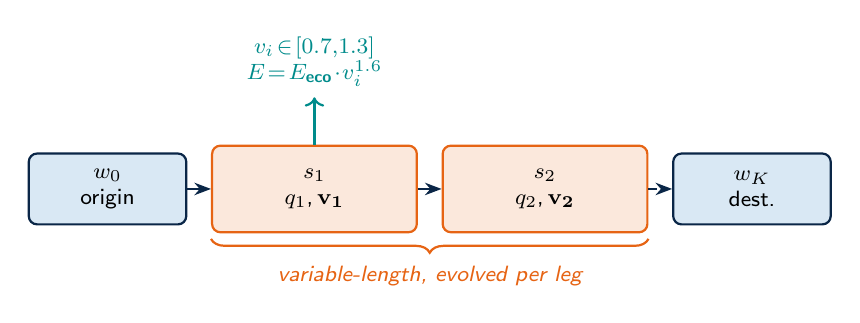
\begin{tikzpicture}[
  gene/.style={rectangle, rounded corners=3pt, minimum width=2.0cm,
               minimum height=0.9cm, align=center, font=\footnotesize,
               draw=PosterNavy, thick, fill=PosterBlue!15},
  stn/.style ={rectangle, rounded corners=3pt, minimum width=2.6cm,
               minimum height=1.1cm, align=center, font=\footnotesize,
               draw=PosterOrange, thick, fill=PosterOrange!15},
  arr/.style ={-{Stealth[length=6pt]}, thick, PosterNavy}
]
\node[gene]                      (w0) {$w_0$\\origin};
\node[stn,  right=0.3cm of w0]  (s1) {$s_1$\\$q_1$,\,$\mathbf{v_1}$};
\node[stn,  right=0.3cm of s1]  (s2) {$s_2$\\$q_2$,\,$\mathbf{v_2}$};
\node[gene, right=0.3cm of s2]  (wk) {$w_K$\\dest.};

\draw[arr] (w0) -- (s1);
\draw[arr] (s1) -- (s2);
\draw[arr,dashed] (s2) -- (wk);

% brace under station genes
\draw[decorate,decoration={brace,amplitude=5pt,mirror},thick,PosterOrange]
     ([yshift=-2pt]s1.south west) -- ([yshift=-2pt]s2.south east)
     node[midway, below=6pt, font=\footnotesize\itshape, PosterOrange]
     {variable-length, evolved per leg};

% velocity callout
\draw[->,PosterTeal,thick] (s1.north) -- ++(0,0.6)
     node[above, font=\footnotesize\bfseries, PosterTeal, align=center]
     {$v_i\!\in\![0.7,\!1.3]$\\$E\!=\!E_\text{eco}\!\cdot\!v_i^{1.6}$};
\end{tikzpicture}
\end{center}

% ── CONVERGENCE CHART ────────────────────────────────────────────────
\hspace*{1.2em}\textbf{EA Convergence --- $Z$-Score vs.\ Generation:}\\[4pt]

\begin{center}
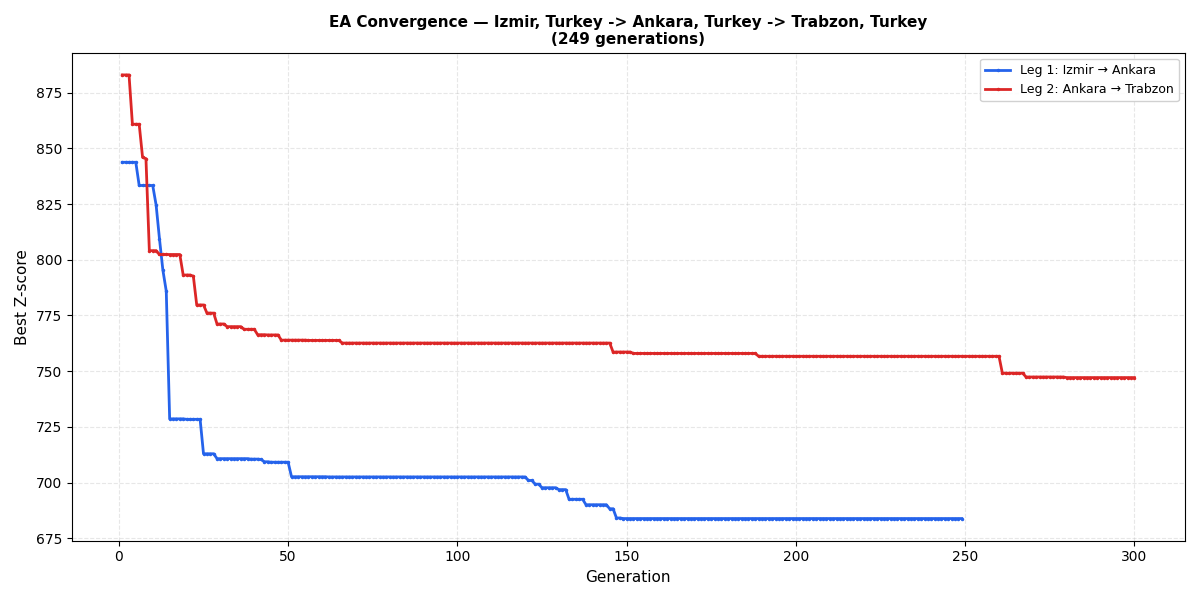
\includegraphics[width=\linewidth]{figures/z-graph.png}
\end{center}

\vspace{0.3cm}

% ── NO-DAG HIGHLIGHT ─────────────────────────────────────────────────
\hspace*{1.2em}%
\begin{minipage}{\dimexpr\linewidth-1.2em\relax}
\begin{infobox}[PosterTeal!10]
\small\textbf{No DAG Restriction.}  Absolute chronological arrival times
$T_{\text{arr},i}$ replace the traditional $i<j$ forward-ordering
constraint.  Since $e_{ij}>0$ for every real road segment, any cycle
degrades SOC monotonically --- infinite loops are \emph{physically}
eliminated without restricting graph topology.
\end{infobox}
\end{minipage}

\vfill
\end{minipage}
\hfill
% ─────────────────────────────────────────────────────────────────────
%  RIGHT COLUMN
% ─────────────────────────────────────────────────────────────────────
\begin{minipage}[t][83cm]{0.31\linewidth}

% ── SECTION 7 — RESULTS ──────────────────────────────────────────────
\section*{7.\ Experimental Results}
\normalsize
\textbf{Scenario Comparison --- Time vs.\ Cost:}\\[4pt]
\begin{center}
\begin{minipage}[c]{0.26\linewidth}
  \footnotesize
  \raggedright
  \textbf{Route:}\\
  İzmir $\to$ Ankara $\to$ Trabzon\\
  (1{,}337\,km)\\[10pt]
  \textbf{Vehicle:}\\
  $\cdot$Tesla Model 3 RWD\\
  $\cdot$ 60\,kWh,\\
  $\cdot$ 135\,Wh/km,\\
  - $B_\text{start} = 80\%$, \\
  - $B_\text{end} = 20\%$
\end{minipage}\hfill%
\begin{minipage}[c]{0.73\linewidth}
  \centering
  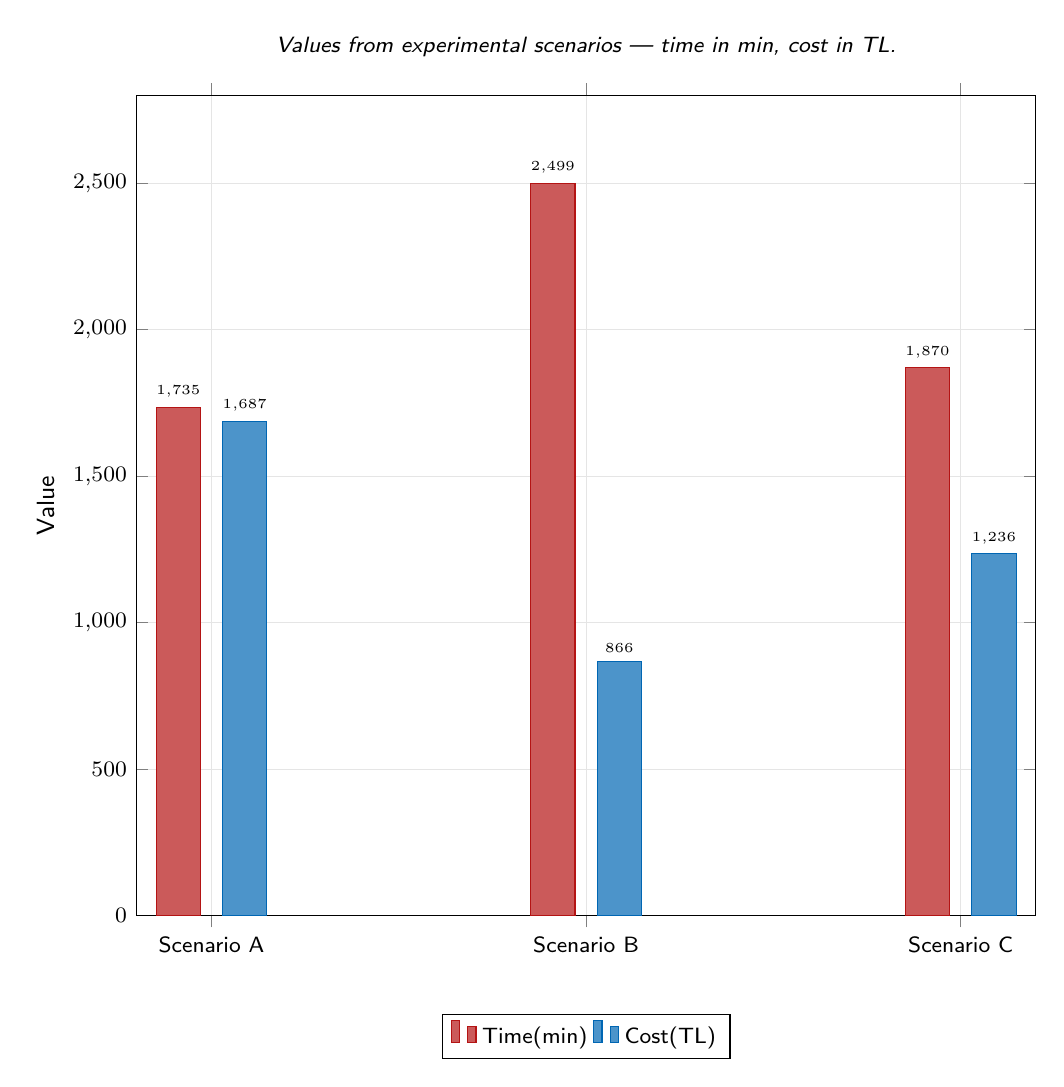
\begin{tikzpicture}
  \begin{axis}[
    ybar=8pt, bar width=16pt,
    width=13.0cm, height=12cm,
    title={\footnotesize\itshape Values from experimental scenarios --- time in min, cost in TL.},
    title style={align=center, yshift=1ex},
    symbolic x coords={A,B,C},
    xtick=data,
    xticklabels={Scenario A, Scenario B, Scenario C},
    ytick={0,500,1000,1500,2000,2500},
    ymin=0, ymax=2800,
    ylabel={\small Value},
    legend style={at={(0.50,-0.12)}, anchor=north,
                  font=\footnotesize, legend columns=2},
    grid=major, grid style={gray!20},
    tick label style={font=\footnotesize},
    label style={font=\footnotesize},
    nodes near coords,
    nodes near coords style={font=\tiny}
  ]
  \addplot[fill=PosterRed!70,  draw=PosterRed]
          coordinates {(A,1735)(B,2499)(C,1870)};
  \addplot[fill=PosterBlue!70, draw=PosterBlue]
          coordinates {(A,1687)(B,866)(C,1236)};
  \addlegendentry{Time(min)}
  \addlegendentry{Cost(TL)}
  \end{axis}
  \end{tikzpicture}
\end{minipage}
\end{center}

\noindent{\small\itshape Note: Scenario B optimizes strictly for travel cost, Scenario A prioritizes travel speed, Scenario C prioritizes comfort and energy efficiency.}

\vspace{0.5cm}

\begin{center}
  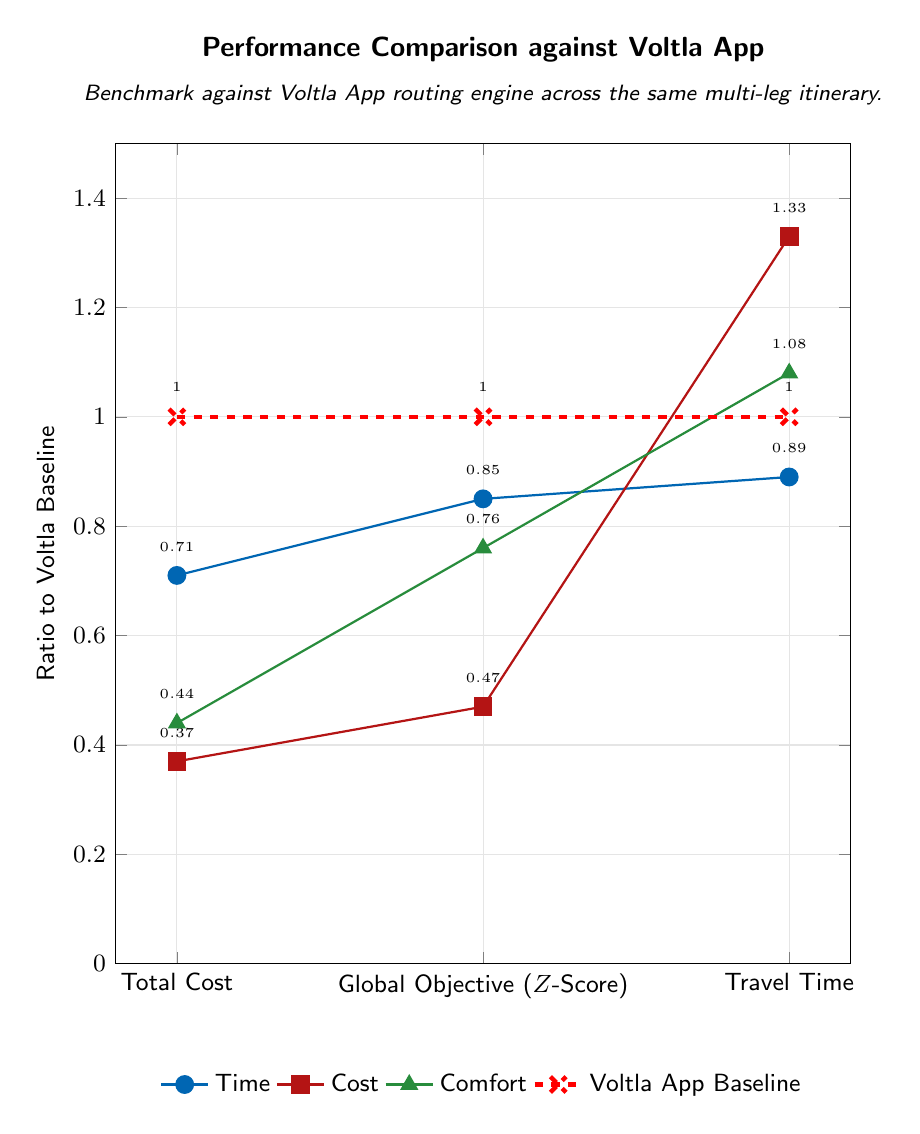
\begin{tikzpicture}
  \begin{axis}[
    width=0.9\linewidth, height=12.0cm,
    title={\textbf{Performance Comparison against Voltla App}\\[4pt]\footnotesize\itshape Benchmark against Voltla App routing engine across the same multi-leg itinerary.},
    title style={align=center, yshift=1ex},
    symbolic x coords={Cost, Z-Score, Time},
    xtick=data,
    xticklabels={Total Cost, Global Objective ($Z$-Score), Travel Time},
    ymin=0, ymax=1.5,
    ylabel={Ratio to Voltla Baseline},
    grid=major, grid style={gray!20},
    legend style={at={(0.5,-0.12)}, anchor=north, legend columns=4, font=\small, draw=none},
    tick label style={font=\small},
    label style={font=\small},
    nodes near coords,
    nodes near coords style={font=\tiny\bfseries, text=black, yshift=5pt}
  ]
  \addplot[color=PosterBlue, mark=*, thick, mark size=3pt] coordinates {(Cost, 0.71) (Z-Score, 0.85) (Time, 0.89)};
  \addplot[color=PosterRed, mark=square*, thick, mark size=3pt] coordinates {(Cost, 0.37) (Z-Score, 0.47) (Time, 1.33)};
  \addplot[color=PosterGreen, mark=triangle*, thick, mark size=3pt] coordinates {(Cost, 0.44) (Z-Score, 0.76) (Time, 1.08)};
  \addplot[color=red, dashed, mark=x, ultra thick, mark size=4pt] coordinates {(Cost, 1.0) (Z-Score, 1.0) (Time, 1.0)};
  
  \legend{Time\hspace{0.8cm}, Cost\hspace{0.8cm}, Comfort\hspace{0.8cm}, Voltla App Baseline}
  \end{axis}
  \end{tikzpicture}
\end{center}

\noindent{\small\itshape Note: Our model includes external variables to evaluate realistic performance.}

% ── SECTION 8 — UI ───────────────────────────────────────────────────
\section*{8.\ User Interface}

\begin{minipage}{0.48\linewidth}
    \centering
    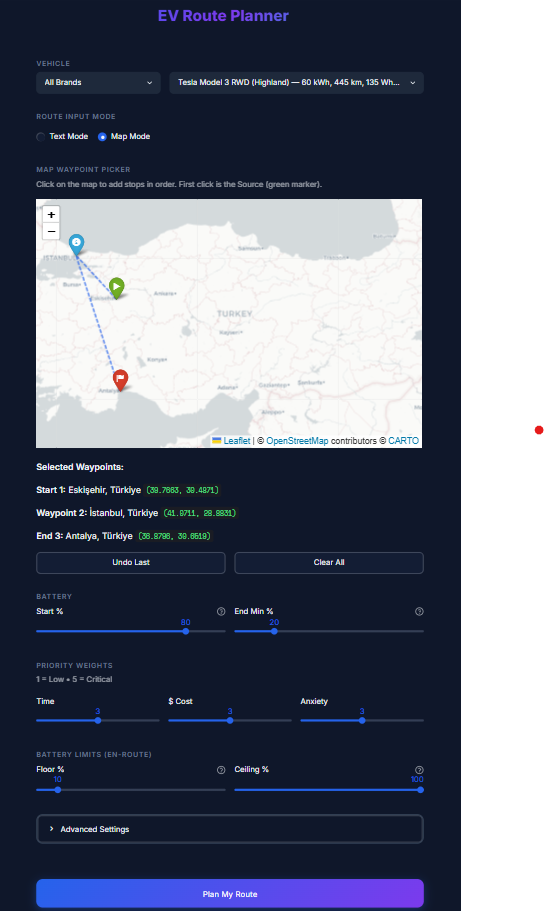
\includegraphics[width=0.70\linewidth]{figures/posterui.png}
    \captionof{figure}{Input Area}
\end{minipage}\hfill
\begin{minipage}{0.48\linewidth}
    \centering
    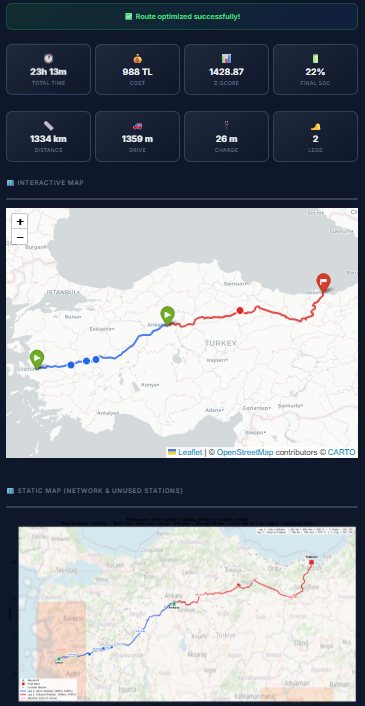
\includegraphics[width=0.70\linewidth]{figures/ui.png}
    \captionof{figure}{Result Area}
\end{minipage}

\vspace{0.2cm}

% ── SECTION 9 — CONCLUSIONS ──────────────────────────────────────────
\section*{9.\ Conclusions \& Future Work}
\begin{itemize}[leftmargin=1.4em,itemsep=2pt]
  \item \textbf{True network topology:} Chronological time-tracking replaces
        DAG constraints, enables real-world loops and backtracking.
  \item \textbf{EA + ALNS hybrid:} Sub-3\,s multi-leg optimisation, viable
        for live consumer web requests.
  \item \textbf{Individual-centric:} First framework targeting individual
        drivers (not fleets) with full UI personalisation.
  \item \textbf{Performance gains:} Outperforms commercial baseline in all
        scenarios, achieving up to \textbf{63\% financial cost savings} and
        \textbf{53\% global objective ($Z$-score) improvement} (under Scenario B).
  \item \textbf{SDG alignment:} Advances \textbf{SDG\,11} (Sustainable
        Cities) and \textbf{SDG\,13} (Climate Action).
\end{itemize}

\vspace{0.3cm}
\textbf{Future work:}
\begin{itemize}[leftmargin=1.4em,itemsep=2pt]
  \item Live IoT station-occupancy telemetry replacing mock $L_i(t)$.
  \item Real-time Open-Meteo weather replacing randomised stress fields.
  \item Non-linear battery thermal throttling \& degradation models.
  \item Game-theoretic multi-vehicle fleet coordination.
\end{itemize}

\section*{10.\ Acknowledgements}
\small
Developed at İzmir Institute of Technology (IZTECH).  Routing powered
by TomTom Developer APIs; infrastructure data from EPDK \textit{\c{S}arj@TR};
vehicle specs from EV Database. 2026

\vfill
\end{minipage}

\end{document}